\documentclass[tikz,border=8pt]{standalone}
\usepackage{amsmath,amssymb}
\usetikzlibrary{arrows.meta,calc,decorations.markings,decorations.pathmorphing,patterns,shapes.geometric,positioning}

\begin{document}
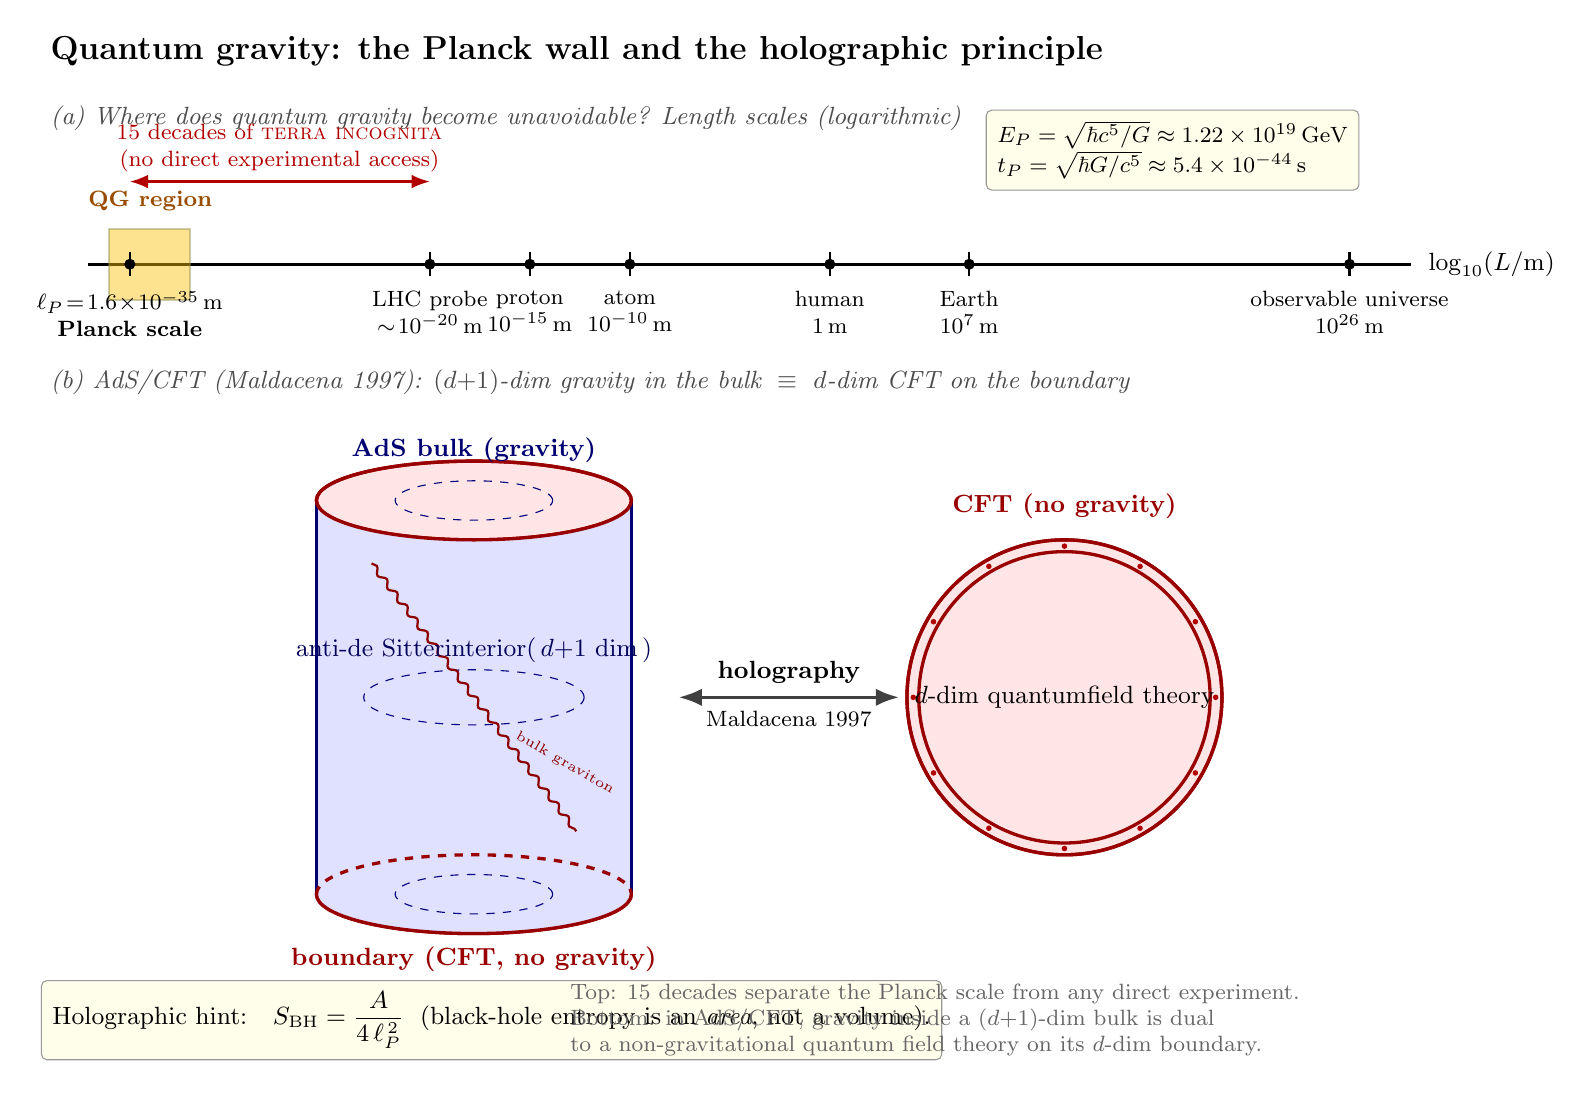
\begin{tikzpicture}[>=Latex,
  axisline/.style={draw=black, very thick},
  tick/.style={draw=black, thick},
  marker/.style={circle, fill=black, inner sep=0pt, minimum size=4pt},
  qgshade/.style={fill=yellow!55!orange, draw=yellow!50!black, opacity=0.45, thick},
  bulkline/.style={draw=blue!45!black, very thick},
  bulkfill/.style={fill=blue!12!white, draw=blue!45!black, very thick},
  cftline/.style={draw=red!60!black, very thick},
  cftfill/.style={fill=red!10!white, draw=red!60!black, very thick},
  arrow/.style={->, thick, black!75}]

  % ===== TITLE =====
  \node[font=\large\bfseries, anchor=west] at (-9.0, 6.7)
    {Quantum gravity: the Planck wall and the holographic principle};

  % =============================================================
  % UPPER PANEL : LENGTH-SCALE LADDER
  % =============================================================

  % Subtitle
  \node[font=\small\itshape, anchor=west, text=black!70] at (-9.0, 5.85)
    {(a) Where does quantum gravity become unavoidable?  Length scales (logarithmic)};

  % Main horizontal axis : x = log10(L/m)  with L in metres
  % Range : -36 to 27   --> draw from x = -9 to x = 9 (1 unit = 7 decades)
  % Use mapping  X = (logL + 4.5) * 0.286  approx  --- let's keep a simple linear mapping:
  %   logL  in [-36, +27]  spans 63 decades; we have 16 cm available (-8 to +8)
  %   scale = 16 / 63 = 0.254 cm per decade
  %   X = (logL) * 0.254
  % Place the axis between x = -8 and +8

  \draw[axisline] (-8.4, 4.0) -- (8.4, 4.0);
  \node[font=\small, anchor=west] at (8.5, 4.0) {$\log_{10}(L/\mathrm{m})$};

  % Helper: tick at a given log-decade
  % We'll define tick positions by hand to keep things readable.

  % ----- Planck length region -----
  % logL = -35  -> X = -35*0.254 = -8.89  (just left of axis, but we put it slightly inside)
  % We'll shift axis mapping: X = (logL + 4) * 0.254 so that human (0) sits roughly at center.
  % logL = -35 -> X = -31 * 0.254 = -7.87
  % logL = -15 -> X = -11 * 0.254 = -2.79
  % logL = -10 -> X = -6  * 0.254 = -1.52
  % logL =   0 -> X =  4  * 0.254 =  1.02
  % logL =   7 -> X = 11  * 0.254 =  2.79
  % logL =  26 -> X = 30  * 0.254 =  7.62

  % QG yellow shading near Planck scale (logL from -36 to -32)
  \fill[qgshade] (-8.13, 3.55) rectangle (-7.11, 4.45);

  % Tick marks and labels
  % Planck length
  \draw[tick] (-7.87, 3.85) -- (-7.87, 4.15);
  \node[marker] at (-7.87, 4.0) {};
  \node[font=\footnotesize, anchor=north, align=center] at (-7.87, 3.78)
    {$\ell_P\!=\!1.6\!\times\!10^{-35}$\,m\\\textbf{Planck scale}};
  \node[font=\footnotesize\bfseries, anchor=south, text=orange!60!black, align=center]
    at (-7.61, 4.55) {QG region};

  % LHC probe  ~ 10^-20 m
  \draw[tick] (-4.06, 3.85) -- (-4.06, 4.15);
  \node[marker] at (-4.06, 4.0) {};
  \node[font=\footnotesize, anchor=north, align=center] at (-4.06, 3.78)
    {LHC probe\\$\sim\!10^{-20}$\,m};

  % Proton ~ 10^-15 m
  \draw[tick] (-2.79, 3.85) -- (-2.79, 4.15);
  \node[marker] at (-2.79, 4.0) {};
  \node[font=\footnotesize, anchor=north, align=center] at (-2.79, 3.78)
    {proton\\$10^{-15}$\,m};

  % Atom ~ 10^-10 m
  \draw[tick] (-1.52, 3.85) -- (-1.52, 4.15);
  \node[marker] at (-1.52, 4.0) {};
  \node[font=\footnotesize, anchor=north, align=center] at (-1.52, 3.78)
    {atom\\$10^{-10}$\,m};

  % Human ~ 1 m
  \draw[tick] (1.02, 3.85) -- (1.02, 4.15);
  \node[marker] at (1.02, 4.0) {};
  \node[font=\footnotesize, anchor=north, align=center] at (1.02, 3.78)
    {human\\$1$\,m};

  % Earth radius ~ 10^7 m
  \draw[tick] (2.79, 3.85) -- (2.79, 4.15);
  \node[marker] at (2.79, 4.0) {};
  \node[font=\footnotesize, anchor=north, align=center] at (2.79, 3.78)
    {Earth\\$10^{7}$\,m};

  % Observable universe ~ 10^26 m
  \draw[tick] (7.62, 3.85) -- (7.62, 4.15);
  \node[marker] at (7.62, 4.0) {};
  \node[font=\footnotesize, anchor=north, align=center] at (7.62, 3.78)
    {observable universe\\$10^{26}$\,m};

  % Bracket explaining the gap from LHC to Planck
  \draw[<->, thick, red!70!black] (-7.87, 5.05) -- (-4.06, 5.05);
  \node[font=\footnotesize, anchor=south, text=red!70!black, align=center] at (-5.97, 5.05)
    {15 decades of $\textsc{terra incognita}$\\(no direct experimental access)};

  % Energy scale annotation (top right of panel a)
  \node[font=\footnotesize, anchor=west, align=left, draw=black!40, fill=yellow!8,
        rounded corners=2pt, inner sep=4pt]
    at (3.0, 5.45)
    {$E_P = \sqrt{\hbar c^5/G} \approx 1.22\times 10^{19}$\,GeV\\
     $t_P = \sqrt{\hbar G/c^5} \approx 5.4\times 10^{-44}$\,s};

  % =============================================================
  % LOWER PANEL : AdS/CFT cartoon
  % =============================================================

  % Subtitle for lower panel
  \node[font=\small\itshape, anchor=west, text=black!70] at (-9.0, 2.5)
    {(b) AdS/CFT (Maldacena 1997): $(d{+}1)$-dim gravity in the bulk $\;\equiv\;$ $d$-dim CFT on the boundary};

  % AdS bulk : drawn as a vertical cylinder (3D-ish look)
  % Centered around (-3.0, -1.5), height = 5, radius = 2.0
  \begin{scope}[shift={(-3.5, -1.5)}]
    % Top ellipse (boundary)
    \draw[cftfill] (0, 2.5) ellipse (2.0 and 0.5);
    % Body of cylinder : sides
    \draw[bulkline] (-2.0, 2.5) -- (-2.0, -2.5);
    \draw[bulkline] ( 2.0, 2.5) -- ( 2.0, -2.5);
    % Bottom ellipse (boundary)
    \draw[cftfill] (0, -2.5) ellipse (2.0 and 0.5);
    % Inside shading (lighter) : two halves
    \fill[blue!12!white] (-2.0, 2.5) -- (-2.0, -2.5) arc (180:360:2.0 and 0.5)
                          -- ( 2.0, 2.5) arc (0:-180:2.0 and 0.5);
    \draw[bulkline] (-2.0, 2.5) -- (-2.0, -2.5);
    \draw[bulkline] ( 2.0, 2.5) -- ( 2.0, -2.5);
    % Re-draw boundary ellipses on top
    \draw[cftline] (0, 2.5) ellipse (2.0 and 0.5);
    % Front part of bottom ellipse
    \draw[cftline] (2.0, -2.5) arc (0:-180:2.0 and 0.5);
    % Back part of bottom (dashed for depth)
    \draw[cftline, dashed] (-2.0, -2.5) arc (180:0:2.0 and 0.5);

    % Light inner curves to suggest curvature
    \draw[blue!50!black, thin, dashed] (0, 2.5) ellipse (1.0 and 0.25);
    \draw[blue!50!black, thin, dashed] (0, 0)   ellipse (1.4 and 0.35);
    \draw[blue!50!black, thin, dashed] (0,-2.5) ellipse (1.0 and 0.25);

    % A curved geodesic in the bulk (representing graviton / closed string)
    \draw[red!55!black, thick, decorate, decoration={snake, amplitude=1pt, segment length=6pt}]
       (-1.3, 1.7) .. controls (0.0, 0.0) .. (1.3, -1.7);
    \node[font=\tiny, anchor=west, text=red!55!black, rotate=-30] at (0.4, -0.4)
       {\,bulk graviton};

    % Labels for the cylinder
    \node[font=\small\bfseries, anchor=south, text=blue!45!black]
       at (0, 2.85) {AdS bulk (gravity)};
    \node[font=\small, anchor=center, text=blue!35!black] at (0, 0.6)
       {anti-de Sitter\\interior\\(\,$d{+}1$ dim\,)};
    \node[font=\small\bfseries, anchor=north, text=red!60!black]
       at (0, -3.05) {boundary (CFT, no gravity)};

  \end{scope}

  % Right side : the boundary CFT shown as a flat circle / ring
  \begin{scope}[shift={(4.0, -1.5)}]
    % Ring (boundary at infinity)
    \draw[cftfill] (0, 0) circle (2.0);
    \draw[cftline] (0, 0) circle (2.0);
    \draw[cftline] (0, 0) circle (1.85);

    % Quantum field "modes" on the ring as small marks
    \foreach \a in {0, 30, ..., 330} {
      \node[circle, fill=red!70!black, inner sep=0pt, minimum size=2pt]
        at (\a:1.92) {};
    }

    \node[font=\small\bfseries, anchor=south, text=red!60!black]
       at (0, 2.15) {CFT (no gravity)};
    \node[font=\small, anchor=center] at (0, 0)
       {$d$-dim quantum\\field theory};
  \end{scope}

  % Double-headed arrow connecting bulk and boundary
  \draw[arrow, very thick, <->] (-0.9, -1.5) -- (1.9, -1.5);
  \node[font=\small\bfseries, anchor=south, align=center]
     at (0.5, -1.45) {holography};
  \node[font=\footnotesize, anchor=north, align=center]
     at (0.5, -1.55) {Maldacena 1997};

  % Bekenstein-Hawking equation as a side-note
  \node[font=\small, anchor=west, align=left, draw=black!40, fill=yellow!8,
        rounded corners=2pt, inner sep=4pt]
    at (-9.0, -5.6)
    {Holographic hint:\quad $S_{\mathrm{BH}} = \dfrac{A}{4\,\ell_P^{\,2}}$
     \;(black-hole entropy is an \emph{area}, not a volume).};

  % Caption for figure (small grey)
  \node[font=\footnotesize, anchor=west, align=left, text=black!60]
    at (-2.4, -5.6)
    {Top: 15 decades separate the Planck scale from any direct experiment.\\
     Bottom: in AdS/CFT, gravity inside a $(d{+}1)$-dim bulk is dual\\
     to a non-gravitational quantum field theory on its $d$-dim boundary.};

\end{tikzpicture}
\end{document}
